\documentclass[a4paper,10pt]{article}
\usepackage[left=2cm,top=2cm,right=2cm,bottom=2cm]{geometry}
\usepackage[utf8]{inputenc}
\usepackage{amsthm}
\usepackage{graphicx}
\graphicspath{ {images/} }


\newcommand{\mN}{{\mathbb N}}
\newcommand{\mZ}{{\mathbb Z}}
\newcommand{\cZ}{{\mathcal Z}}
\newcommand{\fL}{{\mathfrak L}}
\newcommand{\dst}{\displaystyle}

%opening
\title{}
\author{}
\date{}

\begin{document}

\maketitle
Carlos Gallegos\\\\
Quinto Parcial\\\\\\
\textbf{Repaso}\\\\\\
Campo\\\\
Definición: Sea K un conjunto no vacío. Diremos que K es un campo si y solo si existen dos operaciones binarias:\\\\
*: KxK $\rightarrow$ K $\quad\quad$ +: KxK$\rightarrow$K\\\\
tal que para cada a,b,c$\epsilon$K\\\\
a*b, a+b son de K\\\\
a*b=b*a	, a+b=b+a\\\\
(a*b)*c=a*(b*c), a+(b+c)=(a+b)+c\\\\
Existen $e_* , e_+ $ en K tales que $a*e_* = a, a+e_+ =a$\\\\
Existen $f, g \epsilon R$ tales que a*f=$e_*$, a+g=$e_+$\\\\
(a*b)+c=a*c+b*c\\\\\\
Espacio vectorial\\\\
Definición: Sea V un conjunto no vacío y K un campo. Diremos que V es un espacio vectorial sobre K si y solo si existen dos operaciones\\\\
+:VxV $\rightarrow V\quad\quad  \cdot :KxV \rightarrow V$\\\\
tal que para que $u,v,w \epsilon V$ y cada $a,b,c\epsilon K$\\\\
u+v son de V\\\\
(u+v)+w=u+(v+w) y u+v=v+u\\\\
Existe $0\epsilon V$ tal que v+0=v y  existe $z\epsilon V$ tal que v+z=0 \\\\
a$ \cdot$v =ab$\epsilon V$\\\\
(ab)v=a(bv)\\\\
(a+b)v=a(bv) y c(u+v) = cu + cv\\\\
1$\epsilon K$ 1v=v\\\\\
Imágen ilustrativa\\\\
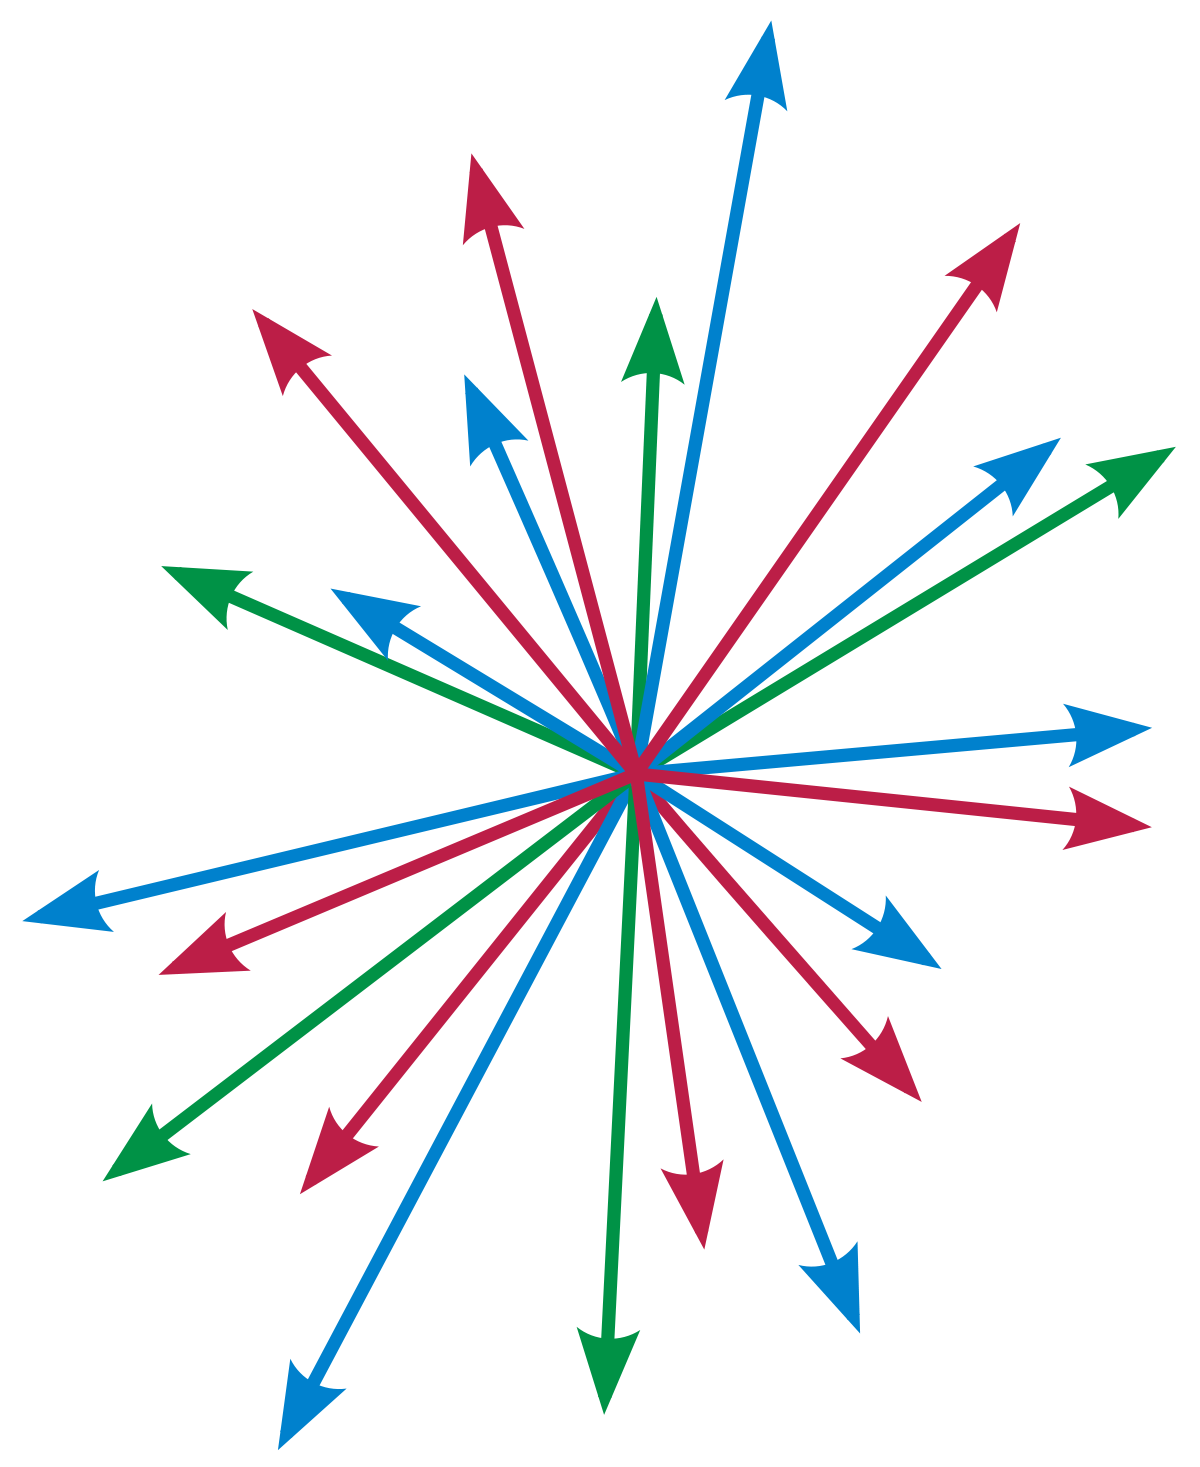
\includegraphics[scale=0.1]{1200px-Vector_space_illust.svg.png}\\\\
Combinación: sean  V espacio vectorial sobre K y u1, . . . , us $\epsilon$V, una combinación lineal de dichos vectores es de la siguiente forma\\\\
 \centerline{$\sum_{i=1}^{s} a_i u_i$}\\\\
con a1,....,ak$\epsilon K$\\\\\\
Base: sean V espacio vectorial sobre K y B $\subset $ V no vacío, diremos que B genera a V si y solo si para cualquier v $\epsilon$ V, v es combinación lineal de vectores en B. Esto es, existen v1, . . . , vn $\epsilon$ B y b1, . . . , bn $\epsilon$ K tales que v = b1v1 + · · · + bnvn.\\\\\\
Teorema: Sea V espacio vectorial finitamente generado sobre el campo K , esto es, existe una conjunto con cardinalidad finita que genera V. Entonces todas las bases de V tienen la misma cardinalidad.\\\\
Sea V finitamente generado, la dimensión de V, denotada por
dimV, es igual a la cardinalidad de una de sus bases. Esto es, si B
es una base para V, entonces\\\\
\centerline{ dimV = $|B|$}\\\\
Donde $|B|$ es la cardinalidad de B.\\\\
Un espacio que no es finitamente generado, se denomina de
dimensión infinita.\\\\\\
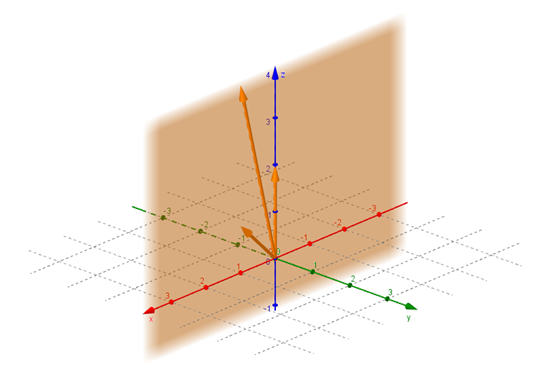
\includegraphics[scale=0.5]{base.png}\\\\
Transformación lineal: sean V, W espacio vectorial sobre el campo K y T : V → W aplicación. Diremos que T es una transformación lineal si y solo si para cada u, v $\epsilon$ V y cada c $\epsilon$ K se cumple que:\\\\
T(u+v)=T(u)+T(v)\\\\
T(cv)=cT(v)\\\\\\
La siguiente tabla nos muestra algunas integrales de repaso para tener en mente, se usarán más adelante para resolver los problemas.\\\\
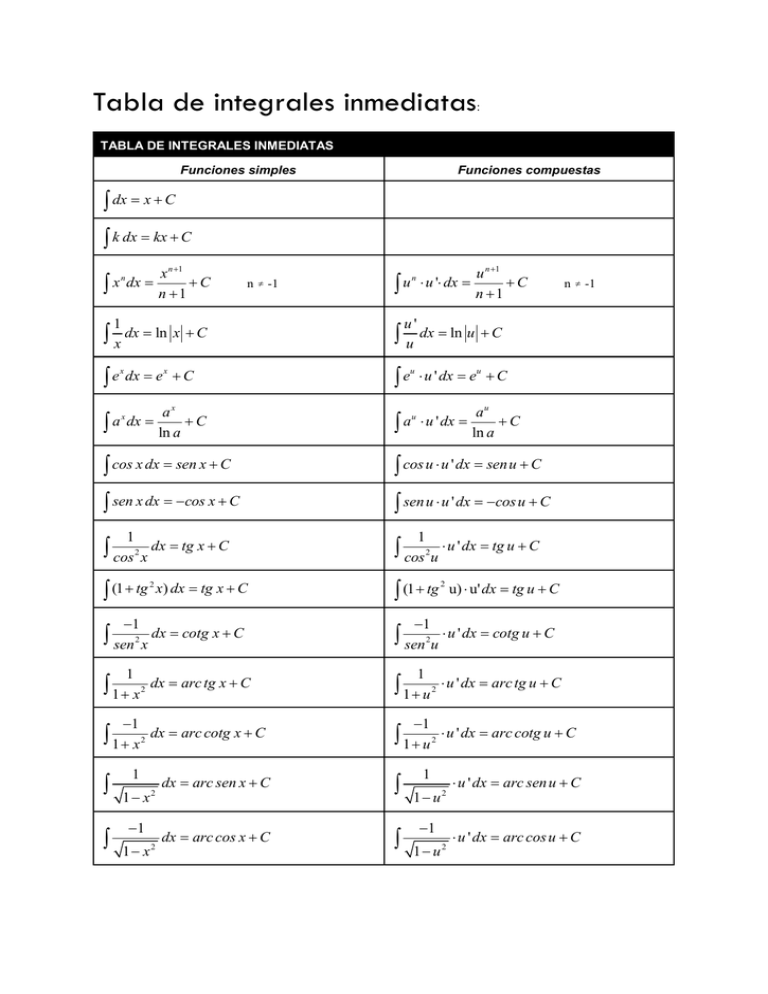
\includegraphics[scale=.6]{integrales.png}\\\\
Ejemplos de resolución de integrales:\\\\
1-$\int \frac{e^{4x}+3}{e^{3x}} dx $\\\\
Primero notamos que podemos separar las fracciones $\int \frac{e^{4x}}{e^{3x}} dx + \int \frac{3}{e^{3x}} dx$\\\\
La primera integral notamos que es directa usando las fórmulas, y en la segunda podemos hacer una cambio de variable de la forma\\\\
\centerline{$e^x + 3[\int e^u]du $ con u=-3x y du = -3dx}\\\\
Hacemos la sustitución y nos queda:\\\\
\centerline{$e^x - e^u = e^x - e^{-3x}$}\\\\
Por transitividad de la igualdad $\int \frac{e^{4x}+3}{e^{3x}} dx = e^x - e^{-3x} +c $ y queda resuelta nuestra integral.\\\\\
2-$\int \frac{x+1}{x^3 + x^2 -6x} dx $\\\\
Se integra por fracciones parciales, para lleos desarrollamos el polinomio:\\\\
\centerline{$\int \frac{x+1}{x(x-2)(x+3)} dx $}\\\\
Entonces encontramos un a, b y c para $\frac{a}{x} + \frac{b}{x-2} + \frac{c}{x+3}$\\\\
Nos queda el sistema $a(x-2)(x+3) + b(x)(x+3) + c(x)(x-2) = x+1$\\\\
Sustituyendo primero x=0, x=2, obtenemos que a=$-\frac{1}{6}$ , b=$\frac{3}{10}$ y c=$-\frac{2}{15}$\\\\
\centerline{$\int [-\frac{1}{6x} + \frac{3}{10(x-2)} - \frac{2}{15(x+3)}] dx $}\\\\
Ahora integramos directamente:\\\\
\centerline{$-\frac{ln}{6} + \frac{3ln(x-2)}{10} - \frac{2ln(x+3)}{15}$}\\\\
Por lo tanto,$\int \frac{x+1}{x^3 + x^2 -6x} dx  = -\frac{ln}{6} + \frac{3ln(x-2)}{10} - \frac{2ln(x+3)}{15} + c $\\\\\\
3-$\int xcosx dx$\\\\
La vamos a integrar por partes, tomamos u=x, u'=1 entonces v'=cos y v=-senx, por lo tanto nos queda\\\\
\centerline{=$xsenx - \int senx = xsenx + cosx$}\\\\
Entonces, nos queda que :\\\\
\centerline{$\int xcosx dx = xsenx - \int senx = xsenx + cosx + c$}\\\\
\newpage
\textbf{Conceptos introductorios}\\\\\\
Ecuación diferencial:\\\\
Definición: Una ecuación que contiene derivadas de una o más variables respecto a una o más variables independientes, se dice que es una ecuación diferencial (ED).\\\\
Ordinaria: si una ecuación contiene sólo derivadas de una o más variables dependientes respecto a una sola variable independiente se dice que es una ecuación diferencial ordinaria (EDO).\\\\
Parcial: Una ecuación que involucra derivadas parciales de una o más variables dependientes de dos o más variables independientes se llama ecuación diferencial parcial (EDP).\\\\
Orden: El orden de una ecuación diferencial (ya sea EDO o EDP) es el orden de la mayor derivada en la ecuación.\\\\
Una ecuación diferencial\\\\
\centerline{$y^{(n)} = f(x,y,y',....., y^{(n)}) $}\\\\
es la forma normal de\\\\
\centerline{$F(x,y,y',.....,y^{(n)})=0$}\\\\
Una ecuación es lineal\\\\
Las derivadas son de y y no de potencias de ella,composici´on
con otras funciones o productos de la derivadas con la variable
independiente\\\\
Las variables ai solo dependen cuando mucho de x.
En caso contrario será no lineal.\\\\\\
Operador lineal:\\\\
Un operador lineal L diremos que es un operador diferencial
lineal si y solo si es de la siguiente forma\\\\
\centerline{$L= \sum_{0}^{n} ai(x)\frac{d^i}{dx^i}$}\\\\
y para constantes c, d y y, y' dos funciones al menos diferenciables hasta orden n, entonces L(cy + $dy'$ )= cL(y) + dL(y').\\\\
Definición de ecuación homogénea:\\\\
Una ecuación lineal\\\\
\centerline{$a_n (x)y^{(n)} + .... + a_0(x)y = g(x)$}\\\\
se denomina homogénea si g(x)=0.\\\\
\centerline{L(y)=$\sum_0 ^n ai(x) \frac{d^i}{dx^i}y =0 $}\\\\
Si g(x) es diferente de cero, entonces es no homogénea.\\\\\\
Solución trivial\\\\
Si tenemos una ecuación de la forma\\\\
\centerline{$a_n (x) y^{(n)} + .... +a_0 (x)y = g(x)$}\\\\
una ecuación diferencial lineal homogénea, entonces y = 0 es
siempre una solución a la ecuación; se denomina la solución trivial.\\\\
También si se tienen u y v soluciones de la ecuación, entonces u + v tambien es solución.\\
El proceso de determinación de las soluciones de una e.d. se llama
resolución o integración de la ecuación.\\\\
Una solución de la ecuación diferencial en que una o más de esas n constantes toman un valor particular se llama solución particular
de la ecuación diferencial La solución con las n constantes
indeterminadas se llama solución general de la ecuación
diferencial.\\\\
Solución implícita y explícita\\\\
Una solución en la cual la variable dependiente se expresa sólo
en términos de la variable independiente y las constantes se
dice que es una solución explícita.\\\\
Se dice que una relación G(x, y) = 0 es una solución implícita
de una ecuación diferencial ordinaria F(x, y
0
, . . . , y
(n)
) = 0, en
un intervalo I, suponiendo que existe al menos una función $\omega$
que satisface la relación así como la ecuación diferencial en I.\\\\\\
Un problema que involucra ecuaciones diferenciales se llama bien
planteado si:\\\\
Tiene solución\\
Su solución es única.\\
La solución depende de modo continuo de las condiciones
complementarias y de todos los parámetros del problema.\\\\
\newpage
\textbf{Ecuaciones diferenciales de primer orden}\\\\
Una solución que contiene una constante arbitraria representa un
conjunto G(x, y, c) = 0 de soluciones llamado familia de
soluciones uniparamétrica. Cuando resolvemos una ecuación
diferencial de orden n F(x, y, y 0 , ..., y (n)
) = 0, buscamos una familia de soluciones n-paramétrica G(x, y, c1, . . . , cn) = 0.\\\\
Una solución de una ecuación diferencial que está libre de la elección de parámetros se llama solución particular.\\\\\\
Variables separables\\\\
Si tenemos una ecuación diferncial $y'=f(x,y)$.\\\\
se puede expresar como una función g(x) que sólo depende de x,
por una función p(y) que solo depende de y, entonces la ecuación
diferencial es separable o se puede resolver mediante separación
de variables. Se tiene la forma:\\\\
\centerline{y'=g(x)p(y)}\\\\
La solución se obtiene el integrar ambos lados de la igualdad\\\\
\centerline{$\int p(y) dy = \int g(x) dx $}\\\\
%acaba clase 26/08
En algunos casos podemos reducir ecuaciones diferenciales a ecuaciones del tipo variables separables.\\\\\\
Ecuaciones exactas:\\\\
Es una ecuación de la forma\\\\ 
$M(x,y)dx + N(x,y) dy = 0$\\\\
Donde las derivadas cruzadas son iguales, es decir, $M_y=N_x$. Es exacta sí sólo sí existe $\omega (x,y)$ tal que $\omega_x (x,y)= M(x,y)$ y $\omega_y (x,y)= N(x,y)$, donde $\omega$ tiene derivadas cruzadas continuas.\\\\\\
%acaba clase 31/08
\centerline{$y'+P(x)y=Q(x)$ , con la condición inicial y(x0)=y0}\\\\\
Sean P y Q funciones continuas en (a,b) que contiene el punto $x_0$. Entonces para cualquier valor inicial $y_0$ existe una única solución y en (a,b) al problema inicial\\\\
\centerline{$\frac{dy}{dx} + P(x)_y =Q(x) \quad y(x_0)= y_0$}\\\\
Donde la solución está dada por\\\\
\centerline{$y(x)=\frac{1}{M(x)}[\int M(x) Q(x) dx + c]$}\\\\
Para un valor específico de c, donde M es el factor integrante.\\\\\\
%acaba clase 02/09
Si L(u) = f(x) es una ecuación lineal inhomogénea con una solución $u_p$  la solución es de la forma $u_h$ + $u_p$, donde L($u_h$) = 0. 
\\\\
Demostración:\\\\
Por definición tenemos que $L(u_p + u_h) = L(u_p) + L(u_h) = f + 0$. Sea $u_{p2}$ otra solución particular a L, notamos que $L(u_{p2} - u_p)=L(u_{p2}) - L(u_p) = f - f = 0$.\\\\
Ahora, ya que $L(u_{p2} - u_p) = 0$, por definición podemos decir que es una solución homogénea, entonces nos queda de la forma $u_{p2} = u_h + u_p$.\\\\
Entonces, podemos obtener una solución general $L(u_g)=f$ si es que conocemos una solución particular y la solución homogénea.
 \\\\\\
Ejemplo de ecuación de Bernoulli\\\\
$\frac{dw}{dt} + 3t^2 w = 6tw^4$ , con y(1)=0\\\\
Por definición, tenemos una ecuación de Bernoulli con P=$t^2w$, Q=$6tw^4$ y n=4.\\\\
Podemos hacer un cambio de variable de la forma z=$w^{1-n} \rightarrow z=w^-3$. Donde el método nos dice que $\frac{dz}{dt} = (1-4)w^-4 \frac{dw}{dt}$. Sustituyendo en nuestra ecuación y simplificando nos queda:\\\\
\centerline{$\frac{dz}{dt} = -3[6t - 3t^2z]$}\\\\
Podemos notar que nos queda una ecuación de variables separables, la cual se resuelve integrando ambos lados de la igualdad. Nos queda:\\\\
\centerline{$\int dz = \int -9t^2 - 18t dt$}\\\\
Las integrales salen directas:\\\\
\centerline{$z = -3t^3 -9t^2  + C$ }\\\\
Ahora vamos a regresar a nuestra variable original $z=w^-3$\\\\
\centerline{$w= \sqrt[3]{\frac{1}{-3t^3 -9t^2  + C}}$}\\\\ 
Ya que tenemos nuestra solución la ecuación, vamos hacer nuestra condición inicial y(1)=0. Para ello susituímos:\\\\
\centerline{$w(1) = \sqrt[3]{\frac{1}{-3 -9  + C}} = 0$}\\\\
Simplificando, nos queda que c=12. Por lo que resolviendo la ecuación de Bernoulli, y con condiciones iniciales w(1)=0, tenemos que la solución es $w= \sqrt[3]{\frac{1}{-3t^3 -9t^2  + C}}$ con c=12.\\\\\\
Funciones homogéneas:\\\\
Una función $f: D \subset R^2 \rightarrow R$ es homogénea de grado n en D sí y sólo sí para cada $t \epsilon R$ se cumple:\\\\
\centerline{$f(tx, ty) = t^n f(x,y)$}\\\\\\
Una ecuación M(x, y) + N(x, y) $\frac{dy}{dx}$ = 0 es homogénea sí sólo sí M y N son funciones homogéneas de grado n.\\\\
Ejemplos:\\
1)x + yy'=0 \\\\
$\rightarrow$ Denotamos M=x y N=y, ahora usamos $t\epsilon R$ y verificamos que cumple M(tx,ty)= tx = $t^1 M(x,y)$. De igual manera se cumple N(tx,ty)= ty = $t^1 M(x,y)$.Por lo que es homogénea de grado 1.\\\\
2)y+xy'=0\\\\
$\rightarrow$ Denotamos M=y y N=x, ahora usamos $t\epsilon R$ y verificamos que cumple M(tx,ty)= ty = $t^1 M(x,y)$. De igual manera se cumple N(tx,ty)= tx = $t^1 M(x,y)$.Por lo que es homogénea de grado 1.\\\\\\
Ejemplos de funciones homogéneas:\\\\
Una función $f: D \subset R^2 \rightarrow R$ es homogénea de grado n en D sí y sólo sí para cada $t \epsilon R$ se cumple:\\\\
\centerline{$f(tx, ty) = t^n f(x,y)$}\\\\\\
Teniendo eso en mente, vamos a probar si son funciones homogéneas.\\\\
1)$f: R^2 \Rightarrow R, (x,y)\Rightarrow xsen(x) + y^2 $ \\\\
Notamos que al hacer f(tx,ty)=$tx sen(tx) + t^2y^2$. Notamos que para que fuera homogénea, se debería cumplir que txsen(tx) fuera igual a tx*tsen(x), lo cual no se cumple, porque tomando t=5 notamos que difieren, y como se debe cumplir para todo t real, no se cumple laigualdad. Por lo que $f(tx,ty)\neq t^n f(x,y)$. Por definición, el inciso 1) no es una función homogénea.\\\\
2)$ g: R^2 \Rightarrow R, (x,y) \Rightarrow x^2y-x^3 + 3y^3$\\\\Notamos que al hacer g(tx,ty)=$t^2 x^2 ty - t^3 x^3 + 3t^3y^3$. Fácilmente se ve que se puede factorizar $t^3$, nos queda g(tx,ty)=$t^3( x^2 y -  x^3 + 3y^3)$.Como $t^3$ está multiplicando a toda la función, al final podemos escribir $t^3 g(x,y)$. Por lo que $g(tx,ty)= t^3 g(x,y)$. Por definición, el inciso 2) es una función homogénea de grado 3.\\\\
3)$h: R^2 \Rightarrow R, (x,y) \Rightarrow \frac{x+y-1}{2x-y+3} $\\\\
Notamos que al hacer h(tx,ty)=$\frac{tx+ty-1}{2tx-ty+3}$. Notamos que no hay manera de factorizar por completo "t"; debido a ello, no podemos decir que $t^n$ está multiplicando a nuestra función h. Por lo que $h(tx,ty)\neq t^n h(x,y)$. Por definición, el inciso 3) no es una función homogénea.\\\\
4)$i: R^2 \Rightarrow R, (x,y) \Rightarrow log(xy)+ e^{xy}$\\\\
Notamos que al hacer i(tx,ty)=$log(t^2xy)+ e^{t^2xy}$. Notamos que no hay manera de factorizar por completo "t", porque no es cierto que $log(t^2xy)$ es igual a $t^2 log(xy)$; debido a ello, no podemos decir que $t^n$ está multiplicando a nuestra función i. Por lo que $h(tx,ty)\neq t^n h(x,y)$. Por definición, el inciso 4) no es una función homogénea.\\\\\\
Ejemplo ecuación exacta:\\\\
Encontrar la función N(x,y) para que la sigueinte ecuación sea exacta. Proporicionar solución:\\
\centerline{ycos(x) + $e^x$ + N(x,y)y' = 0 }\\\\
Primero sabemos que para que sea exacta se debe cumplir que $M_y = N_x$, por lo que se debe cumplir:\\\\
\centerline{$M_y = cos(x) \quad\rightarrow\quad N_x=cos(x)$}\\\\
Por lo que $N(x,y) = \int cos(x) dx = sen(x)+c$\\\\
Entonces, la ecuación diferencial para que sea exacta queda la forma:\\\\
\centerline{ycos(x) + $e^x$ + sen(x)y' = 0}\\\\
Para encontrar la solución tomamos $\omega_x = ycos(x) + e^x$ y $\omega_y=sen(x)y'$ \\\\
Para encontrar $\omega (x,y)$ integramos M y N y la formamos:\\\\
\centerline{$\int Mdx = ysen(x)+e^x + c$ y $\int N dy = ysenx + c$}\\\\
Por lo que $\omega (x,y) = ysenx + e^x$.\\\\
Entonces tenemos que ycos(x) + $e^x$ + N(x,y)y' = 0  es exacta con solución $\omega (x,y) = ysenx + e^x = c$.\\
Notamos que va a ser solución en todo $R^2$.\\\\\\
2. Resolver $y' + sen(x)y^2 -sen(x)y = 0$\\\\
Intentando resolver por variables seperables, primero despejamos y agrupamos terminos:\\\\
\centerline{$\frac{dy}{dx} = -sen(x)y^2 + sen(x)y = sen(x)(y-y^2)$}\\
\centerline{$\frac{dy}{y-y^2}= sen(x) dx$}\\\\
Por lo que resolvemos por variables separables integrando ambas partes:\\\\
$\int \frac{dy}{y-y^2}= \int sen(x) dx$\\\\
$-log(y) + log(y-1) = cos(x) + c $\\\\
Por lo que nos queda como solución implícita $log(y-1)-log(y)   = cos(x) + c $ con $y>1$.\\\\\\
%23 de septiembre
1. Determina si la siguinete función F es homogénea, de ser así,
indica de qué grado es.\\\\
\centerline{ F(x,y) = (x + $\sqrt{y^2 - xy}) - \frac{xy + y^2 }{x} + \frac{x^5}{y^4}$)}\\\\
Primero, tomamos un $t\epsilon R$ y notamos que al hacer F(tx,ty) nos queda:\\\\
\centerline{ F(tx,ty) = (tx + $\sqrt{(ty)^2 - txty}) - \frac{txty + (ty)^2 }{tx} + \frac{(tx)^5}{(ty)^4}$}\\\\
Agrupando términos:\\\\
\centerline{ = $(tx + \sqrt{t^2(y^2 - xy)}) - \frac{t^2xy + t^2y^2 }{tx} + \frac{t^5x^5}{t^4y^4}$}\\\\
Simplificando las divisiones:\\\\
\centerline{= $(tx + t\sqrt{(y^2 - xy)}) - \frac{t(xy + y^2) }{x} + \frac{tx^5}{y^4}$}\\\\
\centerline{ = t(x + $\sqrt{y^2 - xy}) - \frac{xy + y^2 }{x} + \frac{x^5}{y^4}$) = tF(x,y)}\\\\
Por definición, como F(tx,ty) = tF(x,y), y por el grado del exponente, es homogénea de grado 1.\\\\\\
2-Determina si las siguinetes ecuaciones son homogéneas y
proporciona su solución.\\
a) $(x^2 + y^2 ) dx - xydy = 0$\\\\
Si tomamos M(x,y) = $x^2 + y^2$ y N(x,y) = $ -xy$, notamos que son homogéneas de orden 2. 
Por lo que, por definición es homogénea de grado 2. Para resolverla tomaremos cambio de variable u= $\frac{y}{x}$ y se tiene y= ux dy= xdu+udx, por lo que :\\\\
\centerline{ -$u^2x^2dx - u x^3 du = -u^2x^2 -x^2dx$ }\\\\ 
\centerline{-$ - u x^3 du = -x^2dx \rightarrow ux^3 du =  x^2 dx$ }\\\\
Despejando:\\
\centerline{udu = $\frac{1}{x}dx$}\\\\
Tenemos una ecuación de variables separables, la cual resuelve integrando ambos lados de la ecuación:\\\\
$\int u du = \frac{1}{x} dx $\\\\
$ \frac{u^2}{2} = log(x) +c $\\\\
Regresando a nuestra variable original u= $\frac{y}{x}$ nos queda:\\\\
\centerline{$ \frac{(\frac{y}{x})^2}{2} = log(x) +c$}\\\\
Simplificando\\
\centerline{$ y = \sqrt{2x^2 log(x)} + c$}\\\\
Por lo que $ y^2 = 2x^2 log(x) + c$ con $x>0$ es la solución para la ecuación.\\\\\\

\newpage

\textbf{Ecuaciones diferenciales lineales homogéneas de orden superior con coeficientes constantes}\\\\
Definimos:\\\\
a ) Ecuación auxiliar\\\\
Se denomina ecuación auxiliar de L(x)=0 a la ecuación:\\\\
\centerline{$r^n + \sum_{j=0}^{n-1} a_j r^j =0$}\\\\
b ) Polinomio auxiliar\\\\
Al polinomio p(r) = $r^n + \sum_{j=0}^{n-1} a_j r^j$ se le denomina polinomio auxiliar.\\\\
c ) Autovalores propios\\\\
Se denominan autovalores propios a las raíces de la ecuación auxiliar, pueden ser simples o múltiples con el mismo criterio que las correspondientes raíces de la ecuación, siendo el órden el mismo que el órden como raíz correspondiente.\\\\\\
Teorema de existencia y unicidad caso homogéneo:\\\\
Sean a, b, c, x0, y0, y1 $\epsilon$ R, existe una única solución a la ecuación con valores iniciales\\\\
\centerline{$ay'' + by' + cy = 0 \quad\quad y(x_0) = y0 , y'(x0) = y1 $}\\\\
La solución es válida para todo x es real.\\\\
También definimos que un parr de soluciones y1 y y2 son linealmente independientes en el intervalo I si y solo si ninguna de ellas es múltiplo constante de la otra. En caso contrario se denominan linealmente dependientes en I.\\\\
Teorema:\\\\
Si y1 y y2 son dos soluciones cualesquiera a la ecuación diferencial  previamente vista, linealmente independientes en un intervalo I con x0 es I,entonces se pueden determinar constantes únicas C1 y C2 tales que C1y1 + C2y2 satisface el problema con valores iniciales  en I.\\\\\\\
Sean y1, solución a la ecuación diferencial ay00 + by0 + cy = f1 y y2 solución a la ecuación diferencial ay00 + by0 + cy = f2. Entonces, para cualquiera constates c1, c2 $\epsilon$ R la función c1y1 + c2y2 es solución de la ecuación diferencial ay00 + by0 + cy = c1f1 + c2f2.\\\\
Donde f1 y f2 son funciones que dependen de x.\\\\\\
Ejemplo:\\\\
Considerando la función h : R
2 → R con las siguiente regla de
correspondencia, si C es la colección de curvas de nivel de h,
encuentra la familia de curvas ortogonales a C. Además
proporciona una representación gráfica de cada familia de curvas.\\\\
1. $h(x,y)=x^2 -2y$\\\\
Notamos que ya tenemos la ecuación la cual es $x^2 -2y = c$\\\
Para encontrar las curvas ortogonales a c primero derivamos implícitamente para x, nos queda:\\\\
\centerline{$2x -2y' = 0$}\\\\
Como queremos las curvas ortogonales, podemos cambiar y' por $-\frac{1}{y'}$, sustituyendo:\\\\
\centerline{$2x + \frac{2}{y'} = 0 $}\\\\
Ahora simplemente resolvemos la ecuación diferencial, la cual, a simple viste se nota que se puede resolver por variables separables:\\\\
\centerline{$-\frac{2}{y'} = 2x \quad \rightarrow\quad -\frac{1}{y'}= x$}\\\\ 
\centerline{$y'=-\frac{1}{x}$}\\\\
Sabemos que para resolver una ecuación de variables separables integramos ambos lados de la igualdad:\\\\
\centerline{$\int y dy = \int \frac{-1}{x} dx\quad\Longrightarrow\quad y=-log(x) + c0$}\\\\
Por lo que , la familia de curvas ortoganles a c está dada por $y=-log(x) + c0$ con co$\epsilon R$ y $x>0$.\\\\\\
2. $h(x,y)=9(x-1)^2 +4(y+2)^2 $\\\\
Tenemos que la ecuación $9(x-1)^2 +4(y+2)^2 = c$. Donde, para encontrar las curvas ortogonales a c debemos derivar implícitamente para x, nos queda:\\\\
\centerline{$9(x-1) + 4(y+2)y'=0$}\\\\
Como queremos las curvas ortogonales, podemos cambiar y' por $-\frac{1}{y'}$, sustituyendo:\\\\
\centerline{$9(x-1) - 4(y+2)\frac{1}{y}=0\quad \rightarrow \quad y'=\frac{4(y+2)}{9(x-1)}$}\\\\
Para resolver la ecuación diferencial, notamos que es variables separables, la cual se resuelve integrand ambos lados de la igualdad.\\\\
\centerline{$\int \frac{1}{4(y+2)}dy = \int \frac{1}{9(x+1)} dx $}\\\\
Nos queda:\\\\
\centerline{$\frac{log(y+2)}{4} = \frac{log(x+1)}{9} +c0$}\\\\
Por lo que, la familia de curvas ortogonales a c está dada por $\frac{log(y+2)}{4} = \frac{log(x+1)}{9} +c0$ con $c0 \epsilon R$.\\\\\\
3. $h(x,y)=xy$\\\\
Tenemos la ecuación xy=c. Para encontrar las curvas ortogonales primero derivamos implícitamente respecto a x, lo hacemos por regla de la cadena:\\\\
\centerline{y+xy'=0}\\\\
Ahora, como queremos la familia de curvas ortogonales, hacemos el cambio en la pendiente de forma que debemos sustituir y' por $-\frac{1}{y'}$:\\\\
\centerline{$y-x\frac{1}{y'}= 0 \quad\rightarrow\quad x=yy'$}\\\\
Notamos que se resuelve por variables separables, de forma que integramos ambos lados de la ecuación y nos queda como resultado:\\\\
\centerline{$\int y dy = \int x dx   \quad\rightarrow\quad \frac{1}{2} y^2 = \frac{1}{2} x^2  + c0$}\\\\
$y^2 = x^2 + c0$.\\\\
Por lo que, la familia de curvas a c está dada por $y^2 = x^2 + c0$  con $c0\epsilon R $\\\\\\\\
%14 de octubre
Para cada una de las siguientes ecuaciones proporciona la ecuación
lineal homogénea asociada y su solución, encontrar una solución
particular usando coeficientes indeterminados y dar la solución
general.\\\\
1.$\frac{d^2y}{dx^2}+ 3 \frac{dy}{dx} - y = -3x^2$\\\\
Primero debemos encontrar la ecuación lineal homogénea asosiada, la cual notamos que es $y'' + 3y' - y=0 $. Ahora tomamos como ecuación auxiliar $t^2 + 3t - 1 =0$.\\\\
Usamos la fórmula general para encontrar las raíces de nuestra ecuación, en este caso nos quedan dos suliciones las cuales son:\\\\
\centerline{$t1= \frac{-3+  \sqrt{13}}{2} \quad\quad t2=\frac{-3-\sqrt{13}}{2}$ }\\\\
Sabemos que la solución de la ecuación va a estar dada:\\\\
\centerline{$yh(x)= c1 e^{\frac{-3+  \sqrt{13}}{2}x} + c2 e^{\frac{-3-\sqrt{13}}{2}x}$}\\\\
Ahora buscamos una solución particular:\\\\
\centerline{$yp(x)= 3x^2 + 18x +24$ }\\\\
Por úlitmo, sabemos que la solución general está dada por la suma de la solución particular y la solución a la ecuación lineal asociada homogénea. Por lo que tenemos como solución:\\\\
\centerline{y(x) = $3x^2 +18x +24 + c1 e^{\frac{-3+  \sqrt{13}}{2}x} +   c2 e^{\frac{-3-\sqrt{13}}{2}x}$}\\\\\\
2.$-3y'' + y' -y = -2e^{3x}$\\\\
Primero debemos encontrar la ecuación lineal homogénea asosiada, la cual notamos que es $-3y'' + y' - y=0 $. Ahora tomamos como ecuación auxiliar $-3t^2 + t - 1 =0$.\\\\
Usamos la fórmula general para encontrar las raíces de nuestra ecuación, en este caso nos quedan dos suliciones las cuales son:\\\\
\centerline{$t1= \frac{-1+  \sqrt{11 i}}{6} \quad\quad t2=\frac{-1-\sqrt{11i}}{6}$ }\\\\
Sabemos que la solución de la ecuación va a estar dada:\\\\
\centerline{$yh(x)= c1e^{\frac{-1+  \sqrt{11 i}}{6}}+c2e^{\frac{-1-\sqrt{11i}}{6}}$}\\\\
Ahora buscamos una solución particular:\\\\
\centerline{$yp(x)= \frac{2}{25} e^{3x}$ }\\\\
Por úlitmo, sabemos que la solución general está dada por la suma de la solución particular y la solución a la ecuación lineal asociada homogénea. Por lo que tenemos como solución:\\\\
\centerline{y(x) = $ \frac{2}{25} e^{3x} + c1e^{\frac{-1+  \sqrt{11 i}}{6}}+c2e^{\frac{-1-\sqrt{11i}}{6}}$}\\\\\\
3. $ 2\frac{d^2 y}{dx^2} - 4\frac{dy}{dx} + y = 4sen(x) $ \\\\
Primero debemos encontrar la ecuación lineal homogénea asosiada, la cual notamos que es $2y'' - 4y' + 4 y=0 $. Ahora tomamos como ecuación auxiliar $2t^2 - 4t + 4 =0$.\\\\
Usamos la fórmula general para encontrar las raíces de nuestra ecuación, en este caso nos quedan dos suliciones las cuales son:\\\\
\centerline{$t1= \frac{2+  \sqrt{2}}{2} \quad\quad t2=\frac{2-\sqrt{2}}{2}$ }\\\\
Sabemos que la solución de la ecuación va a estar dada:\\\\
\centerline{$yh(x)= c1e^{\frac{2+  \sqrt{2}}{2}}+c2e^{\frac{2-\sqrt{2}}{2}}$}\\\\
Ahora buscamos una solución particular:\\\\
\centerline{$yp(x)= -\frac{4}{17} senx + \frac{16}{17}cosx$ }\\\\
Por úlitmo, sabemos que la solución general está dada por la suma de la solución particular y la solución a la ecuación lineal asociada homogénea. Por lo que tenemos como solución:\\\\
\centerline{y(x) = $ -\frac{4}{17} senx + \frac{16}{17}cosx + c1e^{\frac{2+  \sqrt{2}}{2}}+c2e^{\frac{2-\sqrt{2}}{2}}$}\\\\\\



\newpage
\textbf{Ecuaciones diferenciales no homogéneas con coeficientes constantes}\\\\
Sean A y B dos operadores con coeficientes constantes de orden n
y sean pA y pB sus polinomios característicos respectivamente,
entonces A = B si y solo si pA = pB.\\\\
Si y1, . . . , yn son soluciones linealmente independientes de la
ecuación diferencial L(y) = 0 en el intervalo I; entonces su
wronskiano no es la función nula en I.\\\\\\
Ejemplo de superposición y variación de parámeteros\\\\
Proporciona una solución particular a la siguiente ecuación
aplicando el principio de superposición y el de variación de
parámetros. Luego da la solución general, recordando que dicha
solución debe ser la suma de la particular con la solución de la
homogónea.\\\\
\centerline{$y'' - 2y' + y = log(x) + e^{2x}$}\\\\
Con $x>0$\\\\
Solución:\\\\\
Primero notamos que la ecuación lineal homogénea asociada es $y^2  - 2 y + 1 =0 $ donde las soluciones están dadas de la siguiente forma:\\\\
\centerline{$(y-1)(y-1)= 0 $ con y1=1 y2=2}\\\\
Por lo que la solución a la ecuación lineal con coeficientes constantes es:\\\\
\centerline{yh(x)= $ e^x C1 + xe^2 C2$}\\\\
Ahora vamos a aplicar el principio de supersición y variación de parámetros:\\\\
Primero resolvemos $y'' - 2y' + y =  e^{2x}$ y nos queda como solución particular yp(x)=$Ae^{2x}$ donde y'p=$2Ae^{2x}$ y y''p=$4Ae^{2x}$. Resolviendo el sistema nos queda que A=1 y que yp1(x)= $e^{2x}$.\\\\ 
Ahora para $y'' - 2y' + y =  log(x)$ nos queda el sistema\\\\
\centerline{$v1'(x)e^x + v2'(x)xe^x = 0$}\\
\centerline{$v1'(x)e^x + v2'(x)(e^x + xe^x) = log(x)$}\\\\
Resolviendo por regla de Cramer nos queda $v1'(x)=xlog(x)\frac{1}{e^x}$ y $v2'(x)=log(x)\frac{1}{e^x}$. Por lo que v1 y v2 estáran dadas por:\\\\
\centerline{$v1(x)=\int xlog(x)\frac{1}{e^x}$ y $v2(x)=\int log(x)\frac{1}{e^x}$}\\\\
Entonces la solución particular es yp2(x)={$e^x \int xlog(x)\frac{1}{e^x} +xe^x \int log(x)\frac{1}{e^x}$.\\\\
Ahora por el principio de superposición y variación de parámetros, tenemos que la solución general es la solución particular mas la solución de la ecuación homogénea, por lo que juntando todo nos quead:\\\\
\centerline{yg(x)= yh(x) + yp1(x) + yp2(x)}\\\\
Sustituyendo:\\
\centerline{yg(x)= $e^x C1 + xe^2 C2 + e^{2x} + e^x \int xlog(x)\frac{1}{e^x} +xe^x \int log(x)\frac{1}{e^x}$}\\\\\\
Ejemplo de calculo de polinomios carácterísticos:\\\\
Calcula los polinomios característicos de los operadores L (en
términos del operador D) asociados a las siguientes ecuaciones,
tambien calculas sus raíces.\\\\
1.$\frac{d^5 y }{dx^5} - 2\frac{d^4  y}{dx^4}   - 8\frac{d^3 y}{dx^3}  + 16\frac{d^2 y}{dx^2} - 9\frac{dy}{dx}  + 18y =0$\\\\
Solución:\\\\
El polinomio característico queda como:\\\\
\centerline{L=$D^5 - 2D^4 - 8D^3 + 16D^2 - 9D + 18$}\\\\
Para encontrar las raices vamos a factorizar:\\\\
$D^5 - 2D^4 - 8D^3 + 16D^2 - 9D + 18 = (D-2)(D-3)(D+3)(D^2 + 1)$\\\\
Por lo que las raíces son (2,-3,3,i,-i).\\\\\\
2.$4\frac{d^4  y}{dx^4}   +2\frac{d^3 y}{dx^3} +\frac{dy}{dx} -y =0$\\\\
Solución:\\\\
El polinomio caractéristico queda como:\\\\
\centerline{L=$4D^4 + 2D^3 +D -1 $}\\\\
Para encontrar las raices vamos a factorizar:\\\\
$4D^4 + 2D^3 +D -1 = (D+1)(2D-1)(2D^2+1)$\\\\
Por lo que las raíces son (-1,1/2,$i\frac{1}{\sqrt{2}} , -i\frac{1}{\sqrt{2}}$).\\\\\\


\newpage
\textbf{Soluciones de ecuaciones diferenciales lineales por el método de series de potencias}\\\\
Método del anulador:\\\\
Sea L(y) = g(x) una ecuación diferencial completa (no
homogénea, inhomogénea) donde L es un operador con
coeficientes constates. Este método consiste en encontrar un
operador A con coeficientes constates que anule a la función g, es
decir A(g) = 0. Así, aplicando el operador a la ecuación dada
obtenemos A · L(y) = A(g) = 0, por lo cual, las soluciones de
L(y) = 0 tambien son solución de A(L(y)) = 0. Se resuelve esta
ecuación y luego se escoge las que satisfacen L(y) = g(x).\\\\
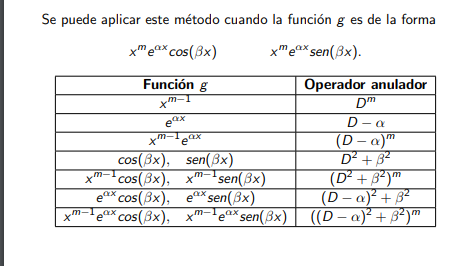
\includegraphics[scale=1]{Anulador.png} \\\\
Cauchy-Euler:\\\\
Se denomina ecuación de Cauchy-Euler (o Ecuación
equidimensional) a una ecuación diferencial lineal de la forma\\\\
\centerline{ $\sum_{j=0}^{n} cj x^j  D^j (y) = g(x)$}\\\\
Con c real y x diferente de cero.\\\\
Obsrevar que el coeficiente de $y^(n)$ es $cnx^n$
la cual se anula en 0. Ahora si procedemos a dividir por ese coeficiente nos resulta que las funciones coeficientes para j$ \epsilon$ {0, . . . , n - 1} no son continuas
en 0. Por lo que la solución se calcula en el intervalo (0, $\infty
$) o bien
en ($-\infty$, 0). En la resolución se puede utilizar dos métodos.\\\\
Método 1:\\\\
Hagamos el cambio de variable x = $e^t$ entonces nuestra ecuación se transforma en:\\\\
\centerline{ $\sum_{j=0}^{n} cj \frac{d^j y }{dt^j} = 0$}\\\\\\
Método 2:\\\\
Se centra en buscar una solución de la ecuación y = $x^r$ con r un número por determinar.\\\\
Tenemos que $D^i(y) = (\prod_{k=0}^{j} (r-k)) x^{r-j}$. Al sustituir esta función y sus derivadas en la ecuación se tiene $x^r$ (q(r)) = 0 siendo q un polinomio con variable r. Ya que $x^r \not =$  0 se tiene que q debe ser 0. Las soluciones de esta ecuación permiten obtener un conjunto fundamental de soluciones.\\\\\\
Ejemplo:\\\\
Resolver la ecuación diferencial xy''' - 2y'' = 0.
Esta es una ecuación de Cauchy-Euler, basta multiplicar a la
ecuación por $x^2$. Realizando el cambio de variable u = y'' se
obtiene la ecuación diferencial xu' - 2u = 0, la cual es una
ecuación lineal de primer orden con solución general u(x)=C1 $x^2$. Al deshacer el cambio de variable se sigue que y''=k1 $x^2$. Al integrar obtenemos\\\\
\centerline{$y(x)= c1 x^4 + c2 x + c3$}\\\\\\
Soluciones en torno a puntos ordinarios\\\\
Se dice que x0 es un punto ordinario de la ecuación diferencial
lineal y'' + P(x)y' + Q(x)y = 0, donde P y Q son funciones
analíticas en una vecindad (entorno) del punto x0; esto es, cada
una de ellas se puede expresar como serie de potencias en una
vecindad de dicho punto. En caso contrario se denomina punto
singular.\\\\\\
Ecuación de Hermite\\\\
\centerline{$y''-2xy'+2py=0 \quad con p\epsilon R$}\\\\
se denomina ecuación de Hermite.\\\\
Para encontrar su solución, primero vemos que 0 es un punto ordinario, puesto las funciones $-2x$ y 2p son analíticas en cero.\\\\




\end{document}